%%%% CS 383 HW #4 - hw4-team3.tex
%%%% Due on BBLearn before 10pm on Friday 3/4/2016


%##########################################################################################################################################################################
% Header
%##########################################################################################################################################################################

\documentclass[11pt]{report}

\usepackage{graphicx}
\usepackage{caption}

\marginparwidth 0.5in 
\oddsidemargin 0.25in 
\evensidemargin 0.25in 
\marginparsep 0.25in
\topmargin 0.0in 
\textwidth 6in \textheight 8.5in

\title{A User's Guide To Squire}
\author{jank6275, mora5651, boss2849, bolt1003, gall7417, brec9824, snev7821, mars2681}

\begin{document}

\maketitle

\tableofcontents


\chapter{Getting Started}

\section{Introduction}
Hello user! You are here because you want to use the exciting new tool Squire! Squire is a developmental tool, allowing you to create projects online, and share them with other users and gain team members to help you complete the project. To get started, you first need to navigate to the Squire website at:  https://squireproject.com/

\section{Create an account}
	\begin{center}
           \includegraphics[width=0.7\textwidth]{Frontpage.png}
    \end{center}
Click on the “Register/Login” button on the front page to reach the registration page.

\pagebreak
	\begin{center}
           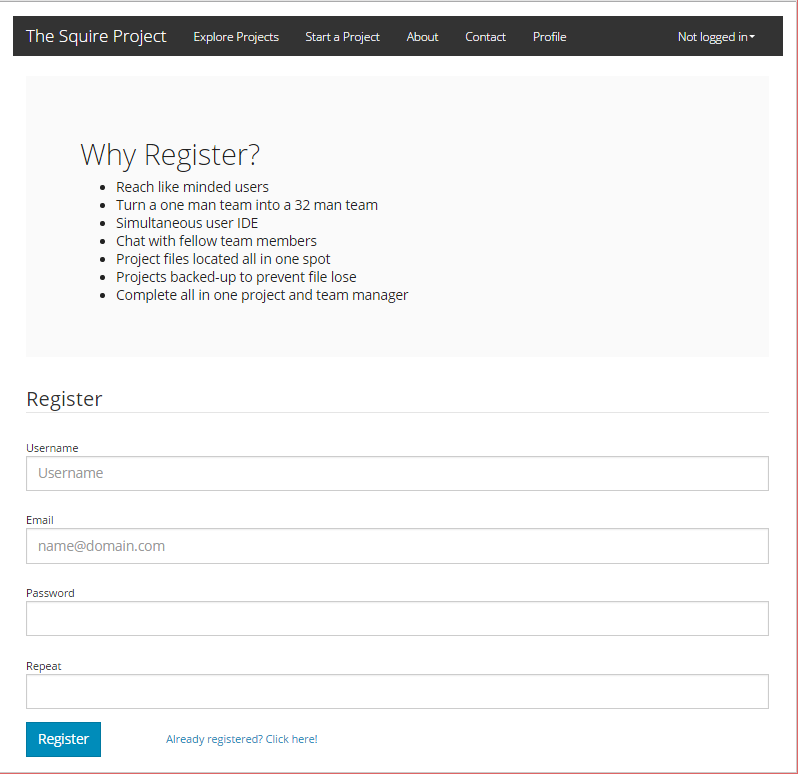
\includegraphics[width=0.7\textwidth]{register.png}
    \end{center}
The register page allows you to create an account. To create an account, enter in a nickname that is at least 6 characters long. This is the name that other users will know you by. Then enter your valid email address. Then enter and reenter a safe password that is at least 6 characters long. Click Register and a confirmation email will be sent to your email account. Once confirmed, you are the brand new owner of a Squire account!

\section{Log In}
	\begin{center}
           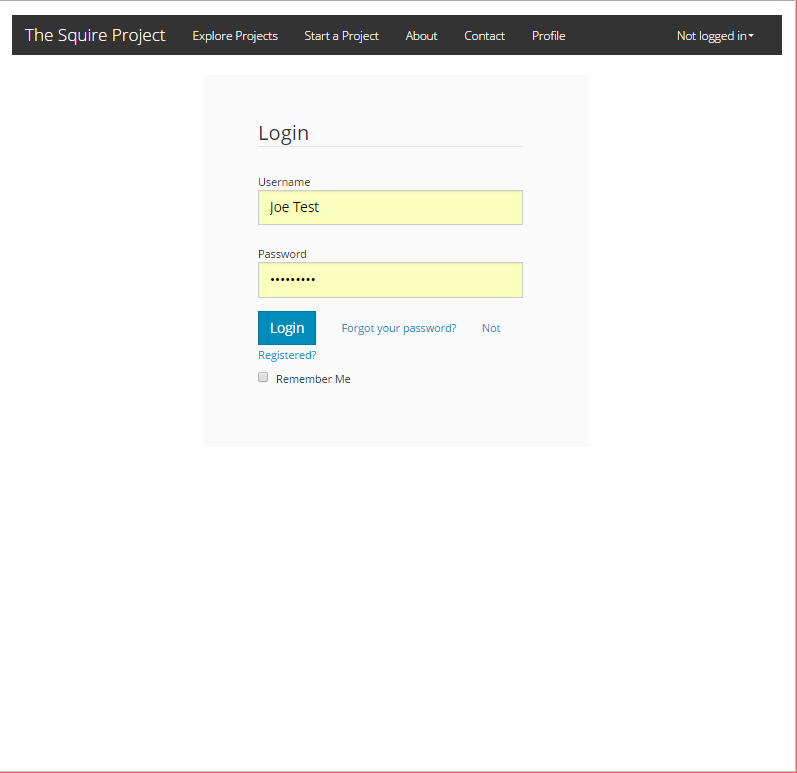
\includegraphics[width=0.7\textwidth]{login.png}
    \end{center}
On the log in page, enter in your username and password, then click Login to access your account. Your browser may automatically remember your credentials, as seen in the picture above. If you forgot your password, click on the link “Forgot your password?”, enter your email address on the following page, and our system will send you a new temporary password.


\chapter{Browsing projects}      
        
\section{Front Page}        	
Once you have registered or have logged in, you will be brought to the main page! This is where you can browse projects, create your own project, or edit your settings

\section{Browse projects}  
	\begin{center}
           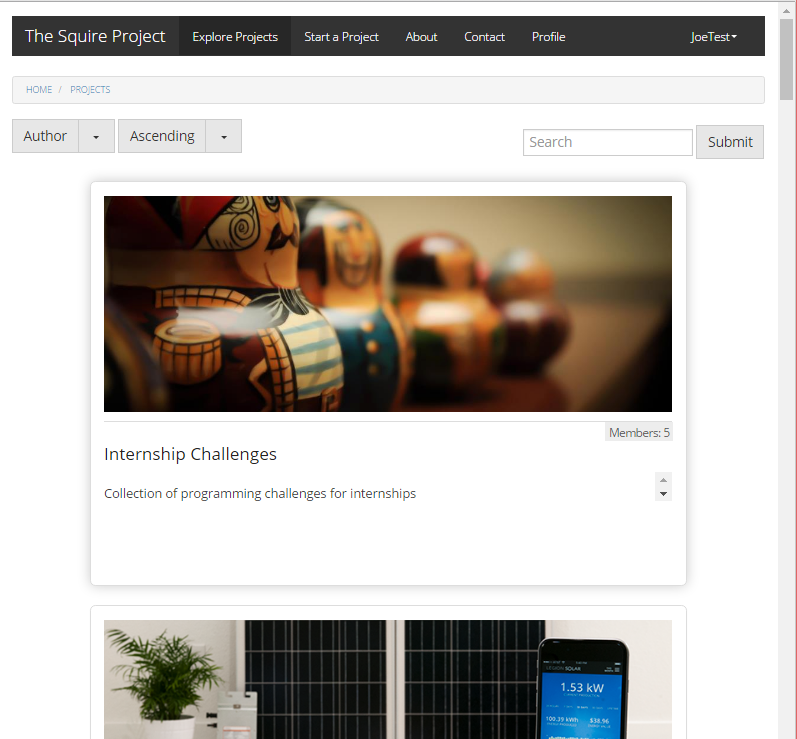
\includegraphics[width=0.7\textwidth]{mainpage.png}
    \end{center}
All projects can be seen on the main page. These can be seen by scrolling down on the main page. To see more projects, you can select another page at the bottom of the screen. To learn more about a project, click on it to be brought to the project page.

\section{Browse Projects By Type}  
To search for a certain kind of project, you can sort all projects by author, title, creation date and last modified date. To sort, click on the sort button in the top left hand side of the page, and select a sorting type from the top down menu. 

\section{Search For Project By Name}  
You can search for a project by it's specific name using the Search bar in the top right hand side of the page. 

\section{Project Page}
	\begin{center}
           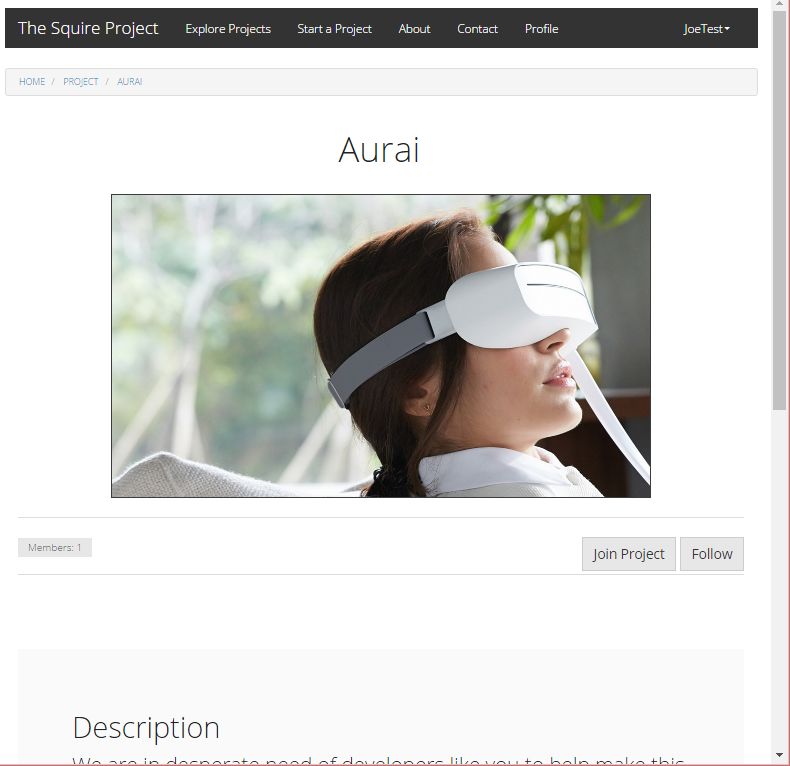
\includegraphics[width=0.7\textwidth]{projectpage_top.png}
    \end{center}
Through project pages, you can learn more about a project, as well as follow, contribute to, and comment on a project. Each project has a picture, a short and a long description to give the user a better understanding of the project.

\section{Follow A Project}
To follow a project, click on the  “Follow” button below the page picture. This will give you updates on the progress of the project, such as new changes or updates to the description. 

\section{Join A Project}
If you would like to contribute code to a project, click on the Join Project button. This will send a join request to the project administrator, who will then decide if you can join or not. Once you are accepted, an access button will be added to this page for you to access the project member's page.

\section{Create A Comment}
	\begin{center}
           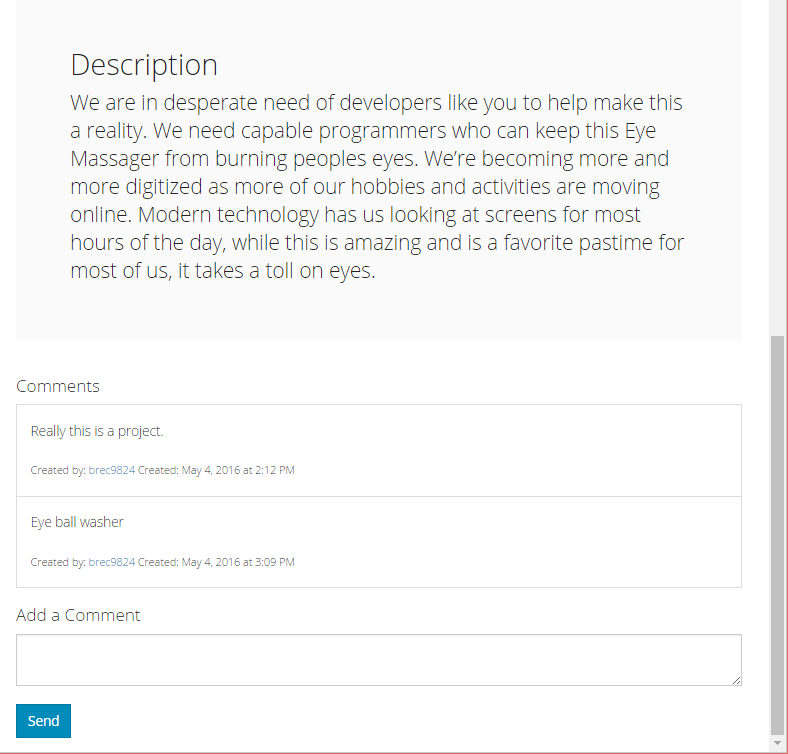
\includegraphics[width=0.7\textwidth]{projectpage_bottom.png}
    \end{center}
At the bottom of the Project page are comments! The Squire community comments are what makes this website such a unique and helpful development tool. To create a comment, type your comment in the “Add a comment” input box and click “Send”. Your comment, along with its timestamp and your username, will then be seen by anyone on this project page! 

\section{Edit Comments}
	\begin{center}
           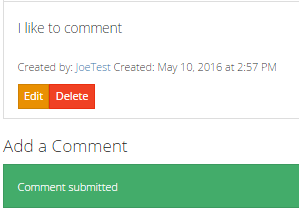
\includegraphics[width=0.7\textwidth]{comment.png}
    \end{center}
If you are unhappy with your comment, you can click “Delete” to remove the comment. Or you can click “Edit” to change your comment. 


\chapter{Creating A Project}

\section{Create Project}
	\begin{center}
           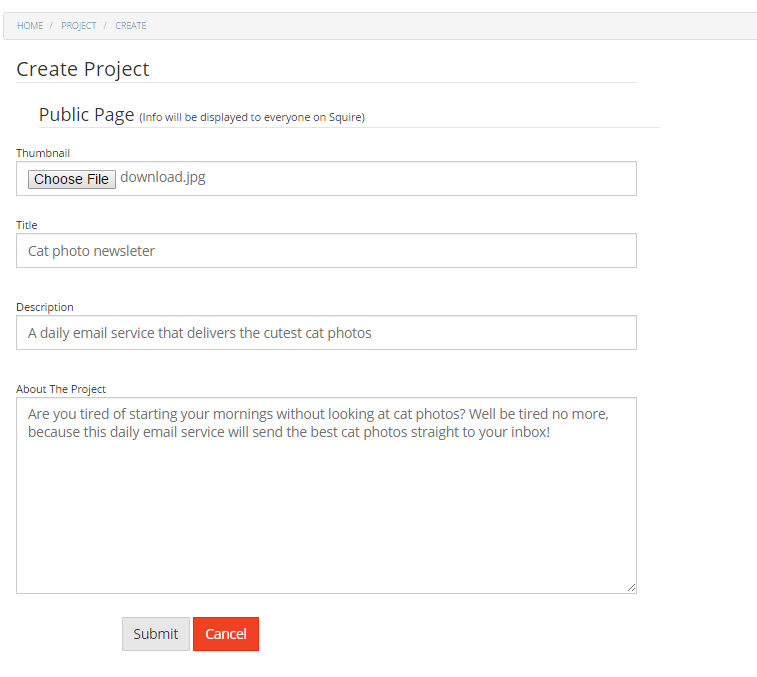
\includegraphics[width=0.7\textwidth]{createproject.png}
    \end{center}
To create a project, click on “Start a project” on the top menu bar to get to the create project page. Every project requires an image, a title, a description of at least 10 characters, and a more detailed description of the project with at least 100 characters. After inputting all these into the Create Project page, and clicking “Submit”, you will be redirected to your Project Page. 

\section{Editing Project Profile}
	\begin{center}
           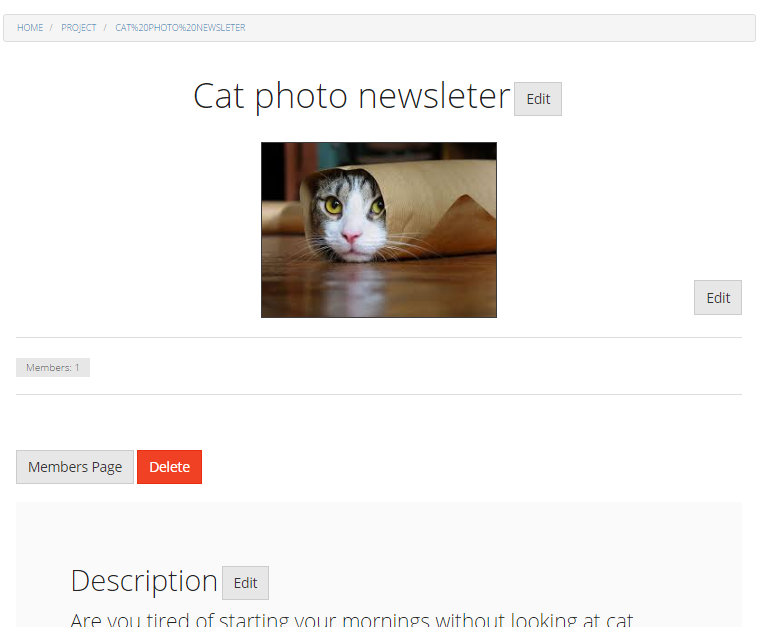
\includegraphics[width=0.7\textwidth]{editprojectpage.png}
    \end{center}
This page is similar to the Project Page, except you can edit the data on this page. To do this, click on the Edit button next to each page element. This page can be re accessed from your profile page by clicking on your Owned Projects. On this page is a button to the Project's Member Page. Click on it to be redirected to it.

\chapter{Project's Member Page}
	\begin{center}
           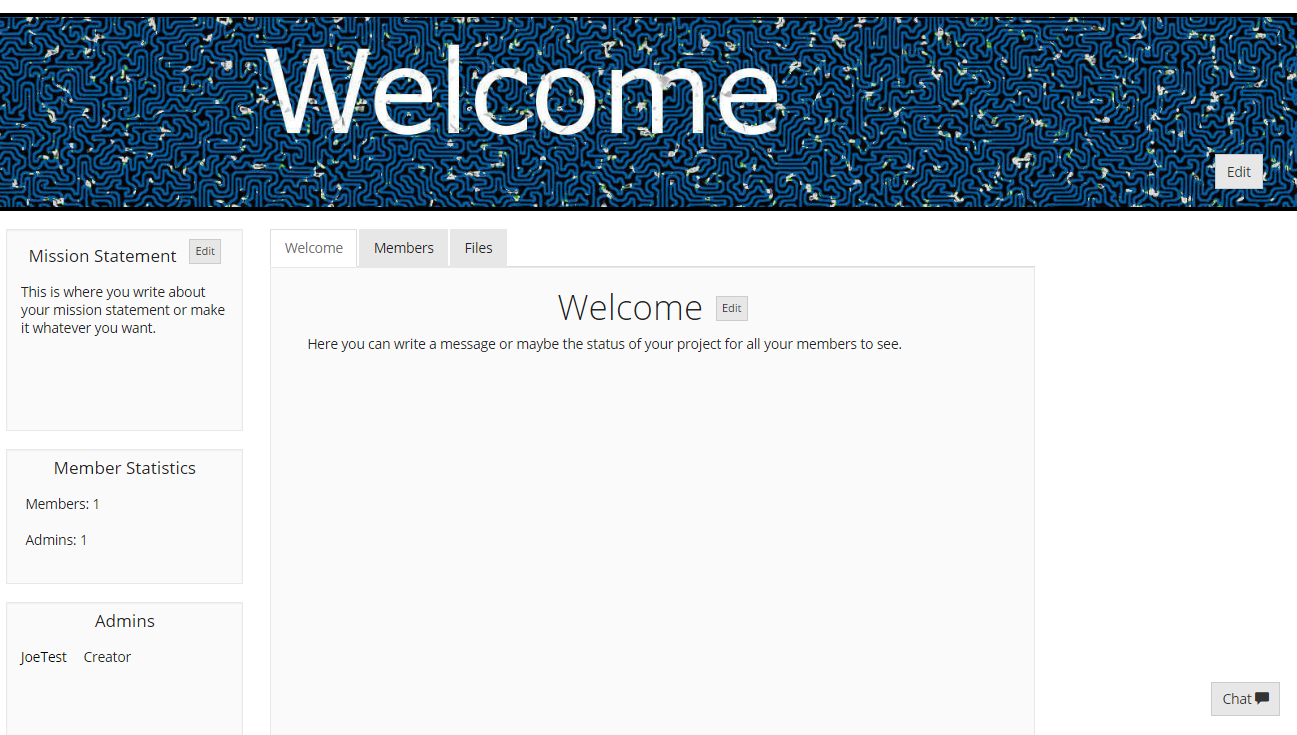
\includegraphics[width=0.7\textwidth]{memberpage.png}
    \end{center}
Only you, and members of your project can see this page. From here, you can accept (or deny) join requests and create the files for your project.

\section{Join Requests}
	\begin{center}
           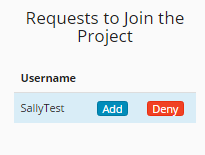
\includegraphics[width=0.7\textwidth]{joinrequest.png}
    \end{center}
Once you get a Join Request, you will see it under “Request to Join the Project.” You can click “Add” to add that User to be a part of your project, or you can click “Deny” to reject their invite.

\section{File Management}
	\begin{center}
           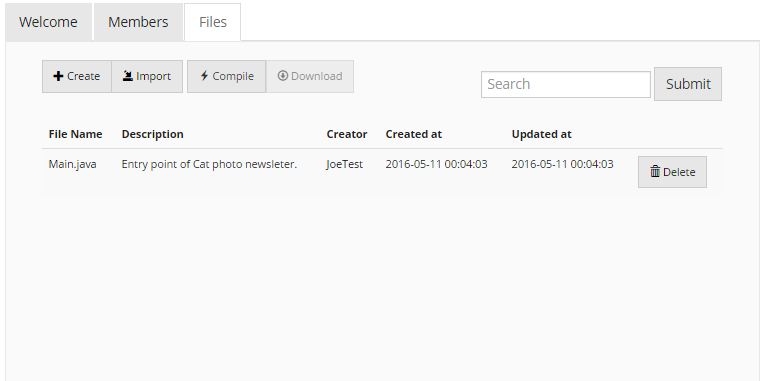
\includegraphics[width=0.7\textwidth]{files.png}
    \end{center}
To start creating some files, click on the “Files” tab. Here, it will show you a list of all your files. Each project has a Main.java file by default. By clicking on this file, you will open it up in Squire’s editor page. To add new files, click either Create to make a new blank file, or Import to import a file from your computer. 

\section{Editor}
	\begin{center}
           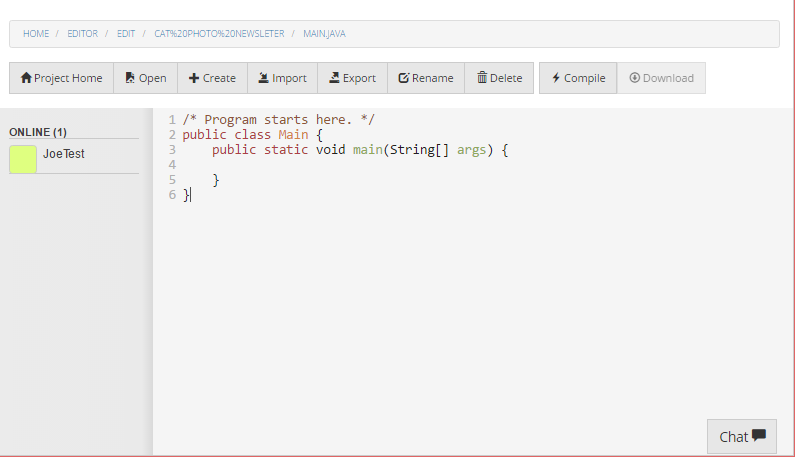
\includegraphics[width=0.7\textwidth]{editor.png}
    \end{center}
The editor page is like most other code editor programs, except it allows two users to work on it at the same time. You can see all the current user's editing on the left, with the color being the color of the font they type. Once you are done typing your code, it will automatically be saved. 

\section{Compiler}
You can compile your code by pressing the “Compile button”. This will export a .jar file that will execute your program. 

\section{Chat}
	\begin{center}
           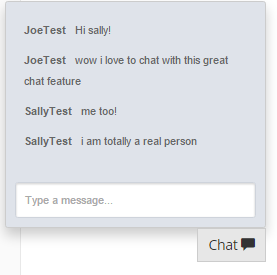
\includegraphics[width=0.7\textwidth]{chat.png}
    \end{center}
Each project has their own chat system built in so members can talk to each other. This feature can be found in the lower right hard corner of the project’s member page, or in the editor. Once it opens, you can see all the chat messages from this project. You can type in your message in the “Type a message” input field. 


\chapter{User Profile}

\section{Profile Tab}   
	\begin{center}
           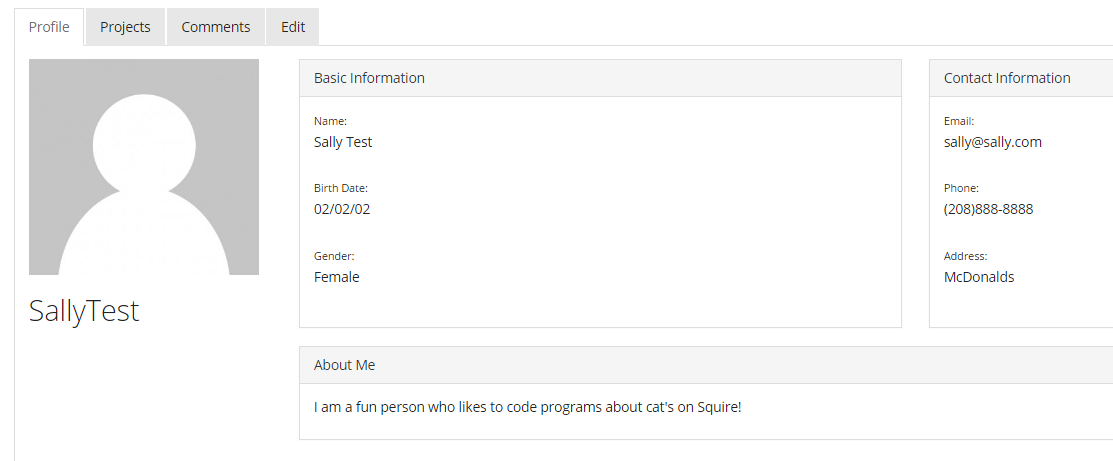
\includegraphics[width=0.7\textwidth]{profile.png}
    \end{center}
Each user has their own profile page. This profile page contains personal information, like an avatar, birthdate, gender, and your bio. By default, this information will be blank, so you will want to edit them in the Edit tab.

\section{Edit Tab}
Edit your information here, and hit submit to change your Profile information. Note that other user's can see this information, so use caution with what information you share.

\section{Projects Tab}
This tab contains all the projects you own. By clicking on one, you will be redirected to it's Edit Project Profile page. From there, you can reach the Project Member's Page.

\section{Comments Tab}
This tab contains all the comments you submitted to project pages. 


\chapter{User Settings}

\section{Settings}
	\begin{center}
           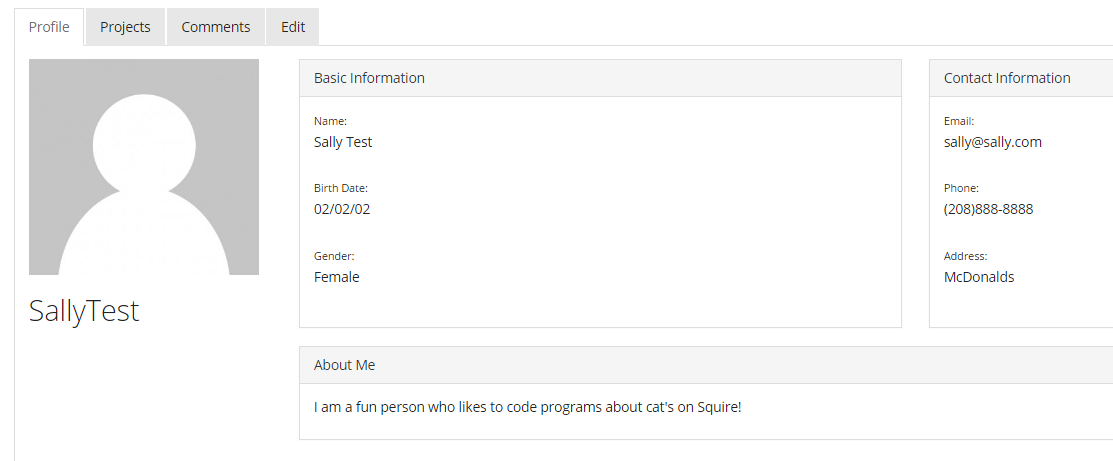
\includegraphics[width=0.7\textwidth]{profile.png}
    \end{center}
Each user has their own settings. You can reach your settings page by clicking on your username in the top right corner, and clicking Settings in the dropdown menu. In this page, you have several options that change the way you edit your project. You can disable the chat feature, change the color of your font, and the type of font. Once you are done editing your settings, click submit and your settings will be saved!


   
\end{document}